\section{System Design}
\label{sec:design}
The runtime exposes named services through two entry paths. Task-mediated calls use the collaboration runtime and a registered agent harness; the harness gives the agent scoped tools for online acquisition, analysis, and control-intent submission. Direct REST or stdio-MCP calls provide verification and integration paths. Both enter the shared dispatcher, while scene configuration supplies context, acquisition bindings, objectives, and write limits.

\begin{figure*}[!t]
\centering
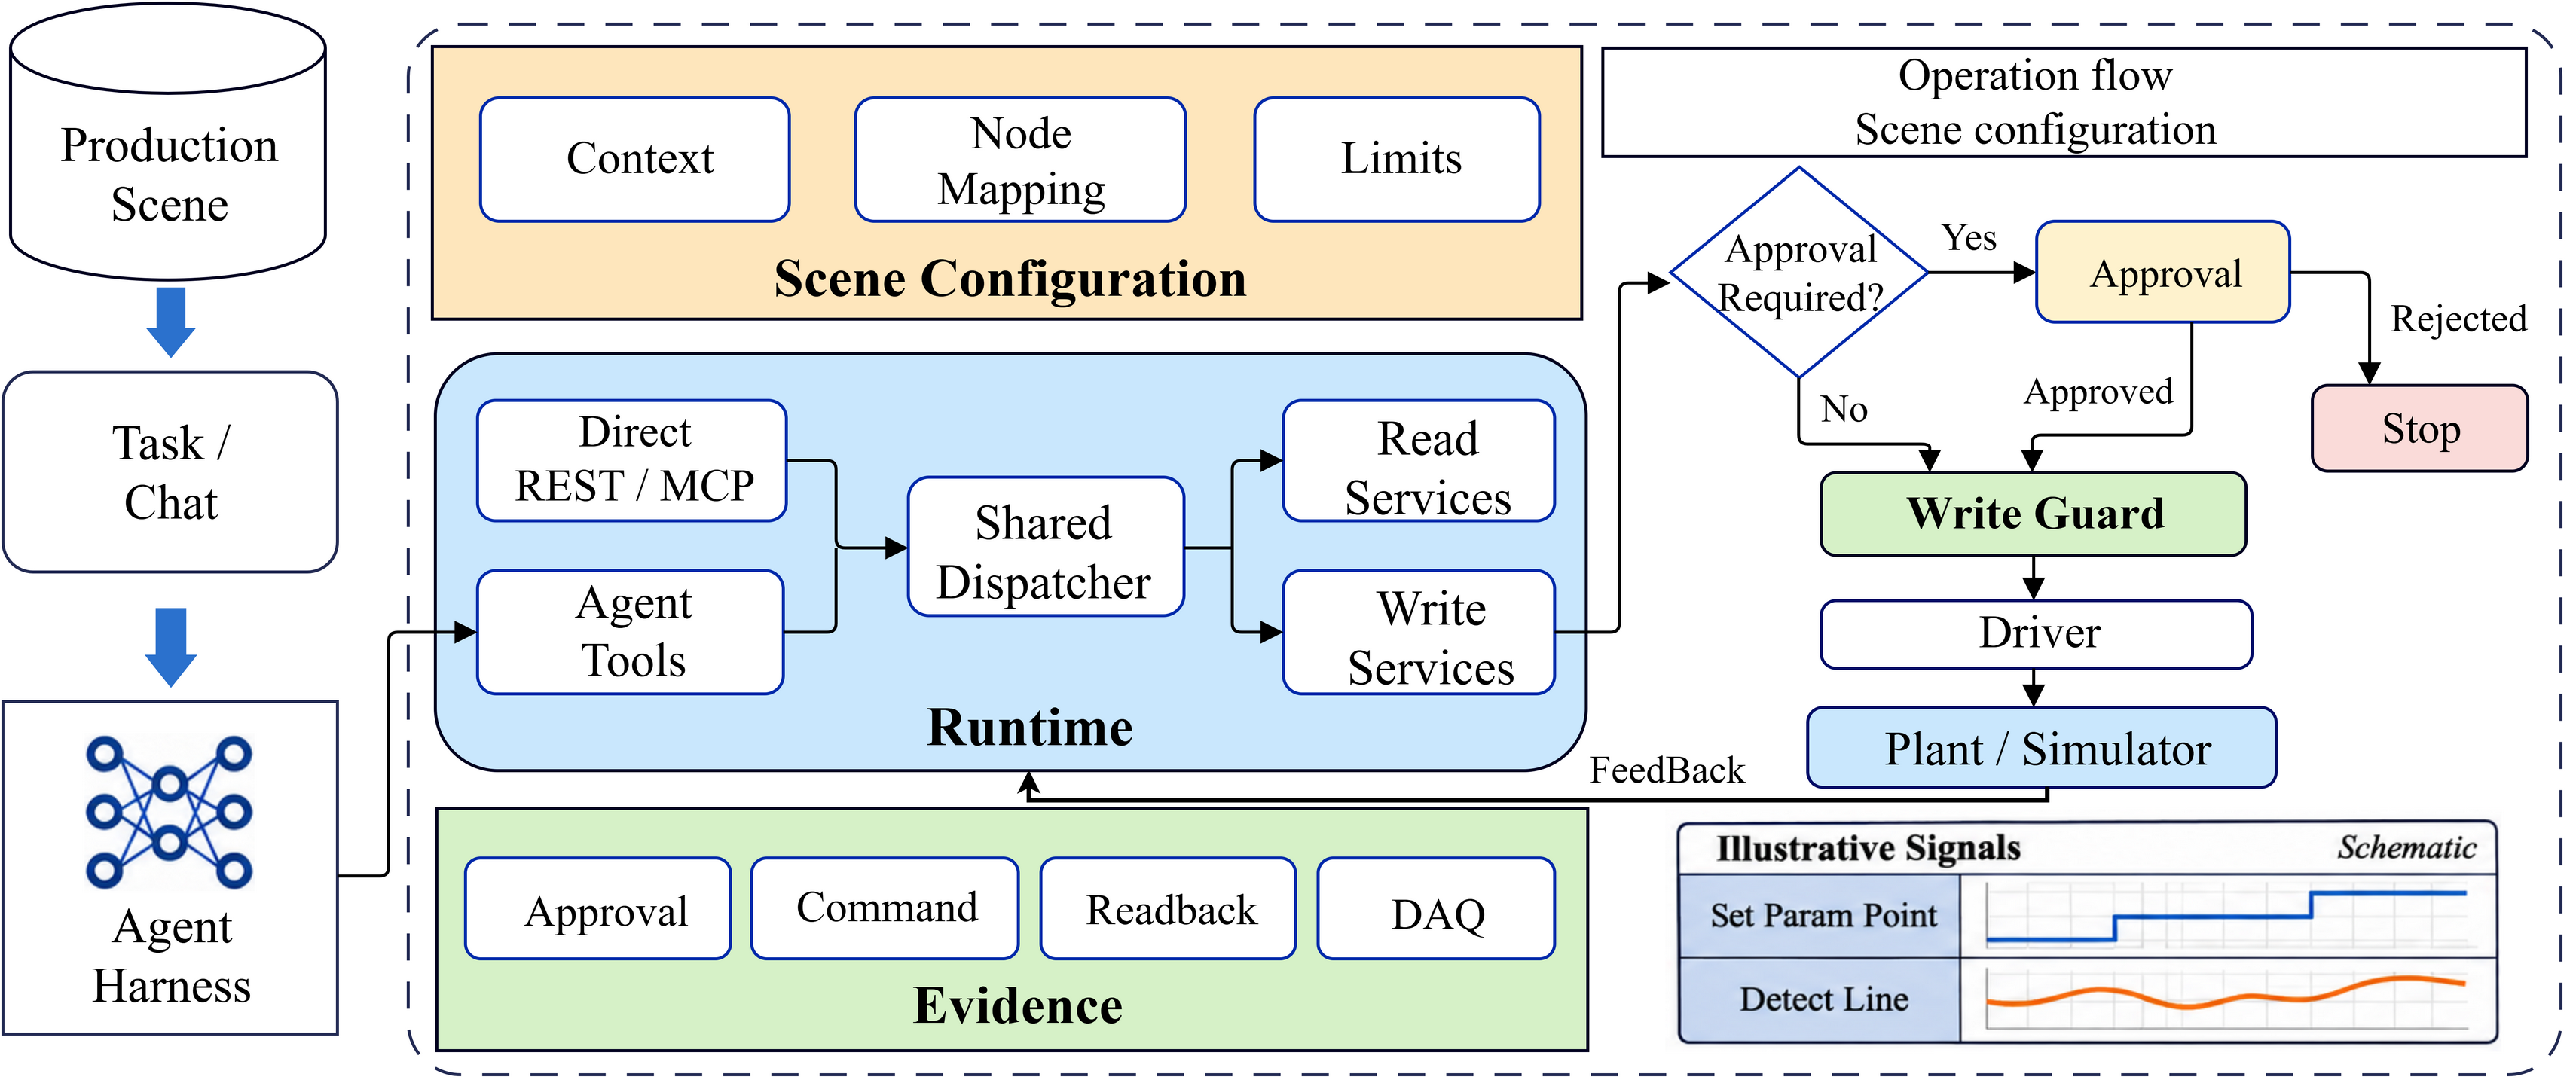
\includegraphics[width=\textwidth]{resources/fig2-user.png}
\caption{Task-mediated and direct tool calls share a dispatcher; a registered agent can acquire observations and submit a control intent, while direct calls provide a verification path. Direct calls need no task. Approved intents undergo route-specific revalidation (omitted here; see Fig.~\ref{fig:hitl}). The no-approval path remains subject to applicable authorization and write guards. Requests rejected by pre-dispatch checks stop before driver dispatch. Feedback and signals are schematic, not measured traces. Approvals, command outcomes, optional readbacks, and later data-acquisition (DAQ) observations are distinct records. In-flight exclusion rejects overlapping writes per node and process; equipment interlocks remain necessary.}
\label{fig:arch}
\end{figure*}

\subsection{Design Rationale and Requirements}
\label{sec:principles}
The runtime must preserve process meaning across heterogeneous drivers, provide a stable contract for registered harness adapters, and check authority and process limits before each control write. It distinguishes acquired process data from command acceptance and later observations. Scene configuration, registered adapters, shared dispatch, route handlers, and service-owned records enforce these boundaries.

The context builder assembles production context and eligible observations for an agent turn. The agent uses them to form a proposal, but context and observations do not grant write authority; the handler resolves live state when the control operation is invoked.

\subsection{Layered Architecture}
\label{sec:layers}
Fig.~\ref{fig:arch} shows the system layers. Task and chat routes use registered harness adapters that provide scoped acquisition and control tools; binding and channel policy constrain available operations. Agent analysis remains distinct from deterministic boundary checks. The figure also shows a schematic feedback path and illustrative signals.

Direct REST agent-tool calls and the stdio-MCP bridge bypass task execution and enter the shared dispatcher. The task route gives the agent context, acquisition targets, and objectives; operation services resolve control mappings and guards. Read/analysis services (DAQ, MES access, retrieval, and optional model services) are separated from write and recipe services. Input/output mappings connect semantic nodes to built-in or plugin drivers, and owning services retain task, command, observation, and configuration records.

\subsection{Scene Configuration as the Integration Boundary}
\label{sec:scene-config}
Scene-specific process semantics are configured before
they are used by an operation. The active line identifies the production context; product
and recipe records supply applicable targets and limits; the run record
provides the current operating state. Semantic nodes bind process variables
to direction-specific acquisition or control mappings, and the driver
registry resolves each mapping to a supported protocol implementation. Here
\emph{semantic} denotes a named process variable with a direction, unit, and
configured mapping; it is not an OPC UA or Asset Administration Shell
information model. Each agent-facing operation is named and typed, so a harness need not
construct protocol-specific messages. A scene using an already registered
driver can supply different context and node mappings behind the same
operation contract. A protocol not present in the registry still requires a
driver adapter; configuration alone does not implement a new protocol.

In the cast-film simulator preset, for example, the MQTT command mapping
\texttt{linespeed-sp} controls line speed in m/min, while the distinct
\texttt{film-thickness} mapping supplies thickness in $\mu$m. An agent can
acquire the thickness observation, compare it with its objective, and propose a
line-speed intent; the runtime admits that intent against the control node's
limits. Sharing MQTT does not make either signal a substitute for the other.

Table~\ref{tab:scene-config} summarizes how the execution path uses the scene
description and distinguishes configuration-time bindings from checks against
live state. The context assembled for an agent turn describes the active scene. Before a
write, the handler resolves the live state required by its route and applies
the current limits. Where a route supports context snapshots, approval is
bound to both the proposal and the context. The command receipt remains
separate from subsequent DAQ observations.

\begin{table*}[!t]
\centering
\caption{Scene configuration elements and their roles in the runtime path.}
\label{tab:scene-config}
\footnotesize
\setlength{\tabcolsep}{5pt}
\begin{tabularx}{\textwidth}{@{}>{\raggedright\arraybackslash}p{0.19\textwidth}>{\raggedright\arraybackslash}p{0.34\textwidth}X@{}}
\toprule
Element & Configured information & Runtime use\\
\midrule
Production context & Line, product, recipe, and run associations & Context construction for a task turn; route-dependent live-state checks before a write\\
Semantic I/O & Process variable, direction, unit, and node mapping & Acquisition uses the read mapping; accepted operations resolve the configured control mapping\\
Driver binding & Supported protocol driver and endpoint configuration & Driver registry selects the protocol implementation after operation checks\\
Operation admission & Engineering, baseline, product, and recipe limits; step and timing rules where configured & Route handler checks the candidate against current bounds and rejects inadmissible requests\\
Approval policy & Whether approval is required and the decision validity window & Pending request binds the proposed action; route-specific checks run after approval\\
Evidence ownership & Command receipt, verification grade, and later DAQ observations & Owning services retain command outcomes separately from process measurements\\
\bottomrule
\end{tabularx}
\end{table*}

\subsection{Cross-Module Execution Flow}
\label{sec:executionflow}
For a task-mediated call, the registered adapter presents a scoped tool
catalog containing acquisition, context, and control operations to the agent.
The agent reads available observations, relates them to the task objective, and
submits a typed intent rather than a protocol-specific message. At the
operation boundary, the shared dispatcher checks the predicates declared for
the named operation before selecting its handler. The handler resolves live
production state, applies route-specific guards and limits, and requests any
required approval before device I/O.

For an industrial operation $u$ by agent $a$ in channel $c$, define the
shared dispatch condition as
\begin{equation}
\mathcal{A}(a,c,u)=\bigwedge_{X\in\mathcal{C}(u)}X(a,c,u).
\label{eq:dispatch-contract}
\end{equation}
In Eq.~(\ref{eq:dispatch-contract}), $S$, $P$, $G$, and $B$ denote invocation scope, current channel policy,
applicable industrial grant, and the agent's binding to referenced resources,
respectively. $\mathcal{C}(u)\subseteq\{S,P,G,B\}$ is the set of predicates
declared for operation $u$; it always contains $S$ and $P$. The grant predicate
$G$ is included when the resolved channel, target line, and owner/grant policy
require it; explicit exemptions omit it. The binding predicate $B$ is included
when the operation declares resource references. An operation that declares
no references omits $B$. Each included check must pass before handler
selection. The policy predicate includes channel tool selection, profile, and duty-separation checks where
configured.

Once these predicates pass, the selected route applies its operational
guards and requests any required approval. For example, an exploration request checks
the control binding and DAQ visibility before entering the governed write
path; an invisible target returns an error before a write. The checks performed
after approval depend on the route; Section~\ref{sec:modules} specifies the
single-node and recipe-operation paths.

For a direct REST agent-tool call, the service establishes $a$ and $c$ before applying
these checks. An agent token must match the requested agent identifier; an
authenticated user must be the channel owner or an administrator. The manager
loads the channel-agent record and rechecks scope and policy, followed by any
applicable grant and binding checks. Handlers resolve live production state
using request identifiers and the owning services.


